\begin{exercise}
(Ramificaciones)
\begin{enumerate}[label=\alph*)]
    \item Considere la serie de potencias
    $$f(z) = 1 + \frac z2 - \frac {z^2} {2^2 \cdot 2!} + \frac {3z^3} {2^3 \cdot 3!} - \frac {5 \cdot 3 z^4} {2^4 \cdot 4!} + \dots$$
    
    \begin{enumerate}[label=\arabic*)]
        \item Muestre que $f$ es holomorfa en el disco unitario $|z| < 1$.
        \item Muestre que $f$ no puede ser extendida de manera holomorfa a $z = -1$.
        \item ¿Puede $f$ ser extendida de manera holomorfa a $\C - \{ -1 \}$? Explique en detalle su argumento.
    \end{enumerate}
    
    \item Considere $P(z, w) = w^3 - (z^2 + 1)$ y sea $w = \phi(z)$ la solución local de $P(z, \phi(z)) = 0$ alrededor del punto $(z, w) = (0, 1)$. Exhiba dos caminos cerrados desde y hasta $z = 0$ tales que, si extendemos $\phi$ analíticamente a lo largo de estos caminos, llegamos a dos soluciones diferentes alrededor de $z = 0$.
\end{enumerate}
\end{exercise}

\begin{solution}
\leavevmode
\begin{enumerate}[label=\alph*)]
    \item Consideremos la curva algebraica $w^2 = z + 1$. Puesto que la derivada parcial $\partial / \partial w$ no se anula en el punto $(z, w) = (0, 1)$, existe una vecindad de este punto en la curva que es la gráfica de una función holomorfa $w = \phi(z)$. Diferenciando implícitamente, tenemos
    $$w' = \frac 1 {2w}$$
    
    Observemos que $w'$ es una función racional de $w$ de grado $-1$. Es decir, el operador $d/dz$ redujo el grado de $w$ en $2$, de $1$ a $-1$. Esto es perfectamente razonable, porque $w^2$ es un polinomio de grado $1$ en $z$. Postulemos que las derivadas superiores de $w$ son de la forma
    $$\frac {w^{(n)}} {n!} = a_n w^{1-2n}$$
    
    Diferenciando esta expresión una vez más, tenemos
    $$
    \frac {w^{(n+1)}} {(n+1)!}
        = \frac {a_n} {n+1} w^{-2n} \frac {dw} {dz}
        = \frac {1 - 2n} {2 + 2n} a_n w^{-1-2n}
    $$
    
    Entonces la sucesión $a_n$ satisface la recurrencia
    $$a_{n+1} = \frac {1 - 2n} {2 + 2n} a_n$$
    
    Dada la semilla $a_0 = \phi(0) = 1$, el resto de la sucesión es
    $$a_{n+1} = \frac {(-1)^n \cdot 1 \cdot 3 \cdot 5 \cdots (2n - 1)} {2^{n+1} \cdot (n+1)!}$$
    
    Los primeros términos de esta solución son
    $$a_1 = \frac 12, \qquad a_2 = -\frac 1 {2^2 \cdot 2!}, \qquad a_3 = \frac 3 {2^3 \cdot 3!}, \qquad a_4 = -\frac {5 \cdot 3} {2^4 \cdot 4!}$$
    
    Por inspección, $f(z) = a_0 + a_1 z + a_2 z^2 + \dots$ es la serie de potencias de $\phi$ centrada en $z = 0$.
    
    \begin{enumerate}[label=\arabic*)]
        \item El radio de convergencia de $f$ es
        $$\liminf_{n \to \infty} \left| \frac {a_n} {a_{n+1}} \right| = \liminf_{n \to \infty} \frac {2n + 2} {2n - 1} = 1$$
        
        Por ende, $f$ es holomorfa en el disco $|z| < 1$.
        
        \item Supongamos por el absurdo que $g$ es una extensión de $f$ holomorfa en $z = -1$. En particular, $g$ es continua en $-1$ y, por ende,
        $$g(-1) = \lim_{z \to -1} g(z) = \lim_{z \to -1} f(z) = 0$$
        
        La derivada de $g$ también es continua en $-1$ y, por ende,
        $$g'(-1) = \lim_{z \to -1} g'(z) = \lim_{z \to -1} f'(z) = \lim_{z \to -1} \frac 1 {2 f(z)} = \frac 10$$
        
        Esto es imposible, porque $1/0$ no es un número complejo bien definido.
        
        \item Supongamos por el absurdo que $g$ es una extensión de $f$ holomorfa en $\C - \{ -1 \}$. Consideremos el camino cerrado $z = e^{i\theta} - 1$, con $\theta \in [0, 2\pi]$. El levantamiento de este camino a la gráfica de $g$ debería ser el camino cerrado $w = g(e^{i\theta} - 1)$. Sin embargo, el levantamiento es $w = e^{i\theta/2}$, que empieza en $w = 1$ para $\theta = 0$ y termina en $w = -1$ para $\theta = 2\pi$. Por ende, no existe ninguna extensión holomorfa de $f$ al plano agujereado $\C - \{ -1 \}$.
    \end{enumerate}
    
    \item Consideremos tres copias del plano complejo $\C_1, \C_2, \C_3$, con coordenadas $z^2$, $z$, $w$, respectivamente. Observemos que $\C_2, \C_3$ son recubrimientos ramificados de $\C_1$, doble y triple, respectivamente.
    
    En $\C_3$, dibujemos los arcos del círculo unitario que nacen en $w = 1$ y desembocan en las otras dos raíces cúbicas de la unidad. Ambos arcos se proyectan a $\C_1$ como el círculo de radio $1$ centrado en $z^2 = -1$, recorrido desde $z^2 = 0$ hasta $z^2 = 0$. Sin embargo, hay una diferencia: en un caso el círculo es recorrido en sentido antihorario, en el otro el círculo es recorrido en sentido horario.
    
    Cada lazo en $\C_1$ puede ser levantado a $\C_2$ de dos maneras diferentes, una por cada rama de la raíz cuadrada. Escogiendo arbitrariamente un levantamiento de cada lazo, obtenemos los lazos buscados en $\C_2$.
    
    El siguiente bosquejo ilustra la situación:
    \begin{figure}[h]
        \centering
        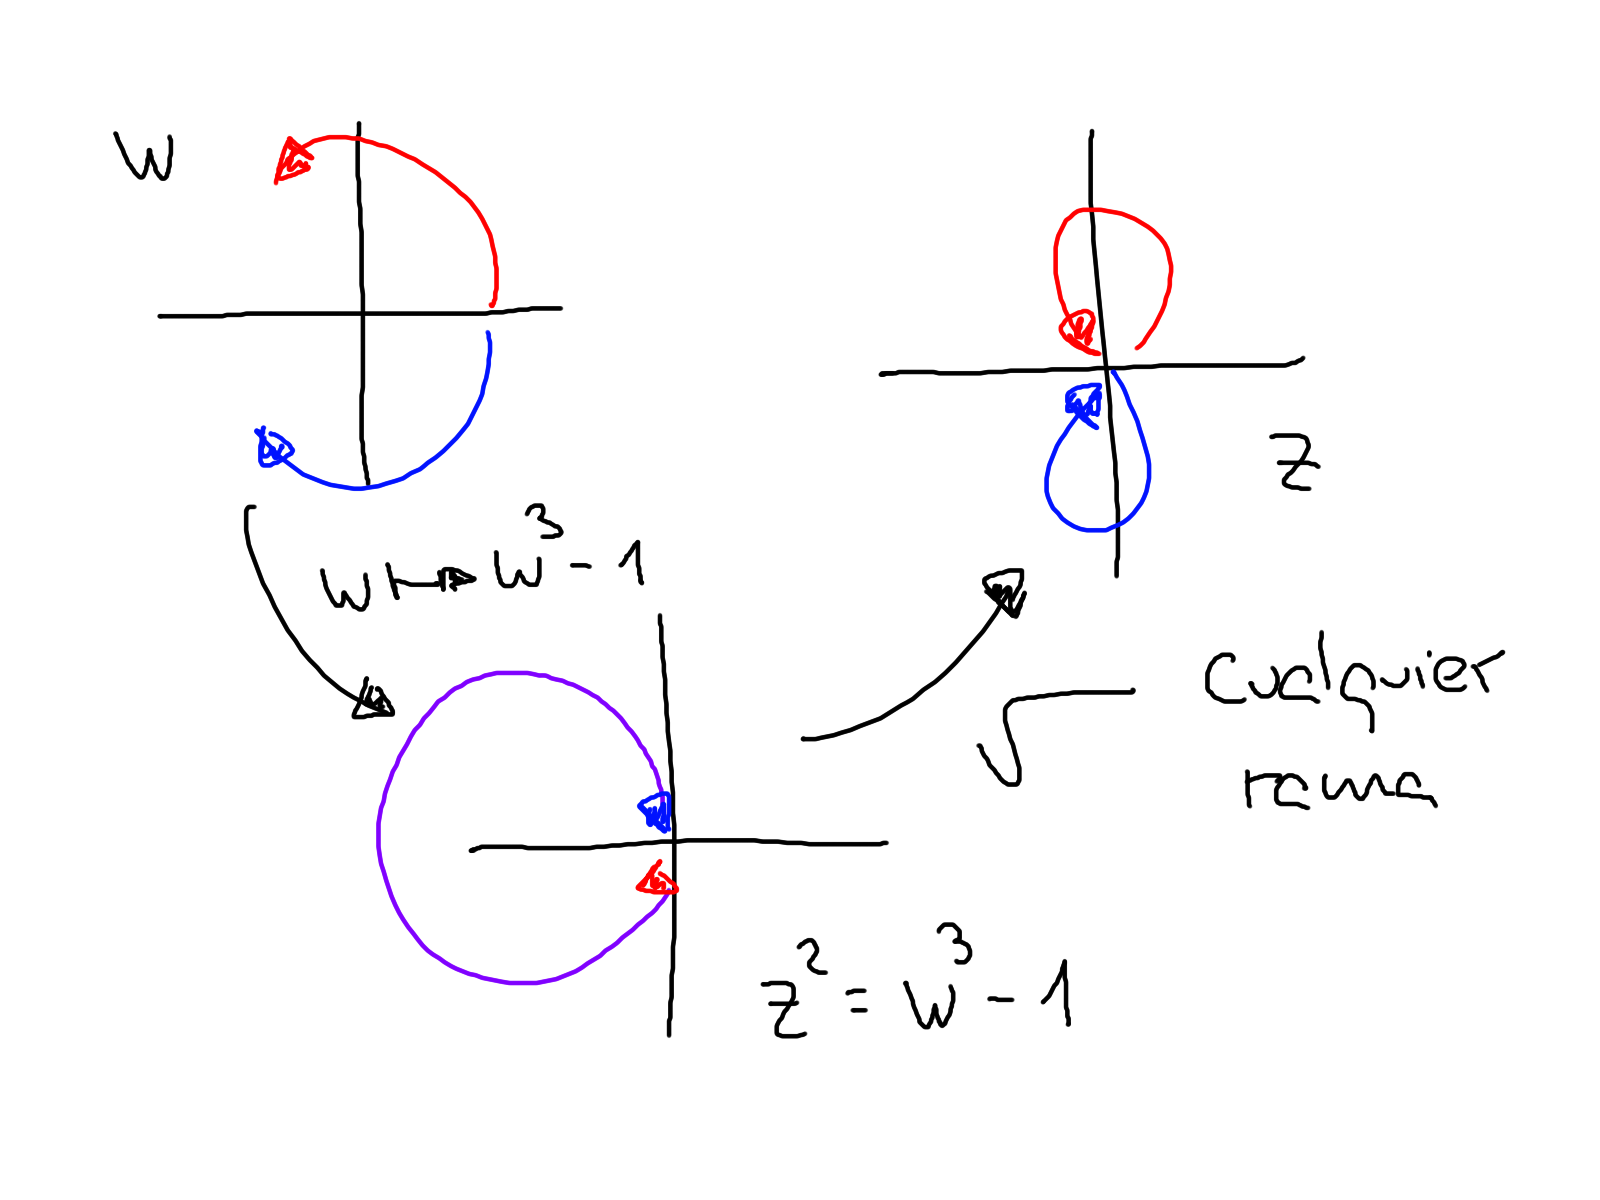
\includegraphics[scale=0.3]{ramification.png}
    \end{figure}
    
    Como se puede observar, los lazos levantados no son diferenciables en $z = 0$. En el gráfico, los lazos parten del origen en direción a $1 \pm i$, pero regresan al origen como si proviniesen de $-1 \pm i$.
\end{enumerate}
\end{solution}
